\section{1D mekanik}

$\overline{x}$ betyder gennemsnit af $x$ over et interval.

Det antages at $y$ er positiv opad i formler for tyngdekraft $g$.

Frit fald er uden luftmodstand og med konstant tyngdeacceleration $g$.

\begin{table}[h]
    \begin{minipage}
        {0.65\textwidth}
        \centering
        \renewcommand{\arraystretch}{1.2} % Increase space between rows
        \begin{tabular}{l|l}
            %% Increase space between rows

            \textbf{Begreb} & \textbf{Formel} \\ \hline
            Displacement & $\Delta x = x-x_0$ \\
            Total Displacement & $\Delta x_{total} = \sum \Delta x_i$ \\
            \\
            Average Velocity & $\overline{v} = \frac{\Delta x}{\Delta t} = \frac{v_0 + v}{2}$ \\
            Instantaneous Velocity & $v(t) = \frac{dx}{dt}$ \\
            \\
            Average Speed & $\overline{s} = \frac{\text{Distance}}{\Delta t}$ \\
            Instantaneous Speed & $s = |v(t)|$ \\
            \\
            Average Acceleration & $\overline{a} = \frac{\Delta v}{\Delta t}$ \\
            Instantaneous Acceleration & $a = \frac{dv}{dt}$ \\
            \\
            Position & $x = x_0 + \overline{v} t$ \\
            Velocity & $v = v_0 + \overline{a} t$ \\
        \end{tabular}
    \end{minipage}
    \hfill
    \begin{minipage}
        {0.3\textwidth}
        \centering

        \textbf{Konstant acceleration}
        \begin{align*}
            v &= v_0 + at \\
            x &= x_0 + v_0t + \frac{1}{2}at^2 \\
            v^2 &= v_0^2 + 2a(x-x_0)
        \end{align*}
        \vspace{2em} \\
        \textbf{Frit Fald}
        \begin{align*}
            g &\approx 9.81 \text{ m/s}^2 \\
            v &= v_0 - gt \\
            y &= y_0 + v_0t - \frac{1}{2}gt^2 \\
            v^2 &= v_0^2 - 2g(y-y_0)
        \end{align*}
    \end{minipage}
\end{table}

\textbf{Integration}
\begin{align*}
    v(t) &= \int a(t) dt + v_0 \\
    x(t) &= \int v(t) dt + x_0 
\end{align*}

Fart er absolut hastighed, og hastighed er fart med retning.

$n$ km/h $\approx$ $\frac{n}{3.6}$ m/s

\subsection{Enheds-omregning}
\begin{align*}
    1 \text{ m/s} = 3.6 \text{ km/h} &\iff
    1 \text{ km/h} = \frac{1}{3.6} \text{ m/s} \\
    1 \text{ m/s}^2 = 12.96 \text{ km/h}^2 &\iff
    1 \text{ km/h}^2 = \frac{1}{12.96} \text{ m/s}^2 \\
    1 \text{ radian} = \frac{180}{\pi} \text{ grader} &\iff
    1 \text{ grad} = \frac{\pi}{180} \text{radianer} \\
\end{align*}

\newpage
\section{3D mekanik}

Formlerne for 3D mekanik virker også for 2D mekanik ved at undlade $z$-komponenten.

Når bevægelse i flere dimensioner opdeles i komponenter kan formlerne for hver komponent behandles som 1D mekanik, og de samlede vektorer kan findes ved at kombinere komponenterne.

\subsection{Bevægelse}

\textbf{Position, Hastighed of Acceleration}
\begin{align*}
    \vec r(t) &= x(t) \hat i + y(t) \hat j + z(t) \hat k \\
    \\
    \vec v(t) = \frac{d \vec r(t)}{dt} &= \frac{d x(t)}{dt} \hat i + \frac{d y(t)}{dt} \hat j + \frac{d z(t)}{dt} \hat k \\
    \\
    \vec a(t) = \frac{d \vec v(t)}{dt} &= \frac{d v_x(t)}{dt} \hat i + \frac{d v_y(t)}{dt} \hat j + \frac{d v_z(t)}{dt} \hat k \\
\end{align*}

\textbf{Displacement, og gennemsnitlig hastighed og acceleration}
\begin{align*}
    \Delta \vec r &= \vec r(t_2) - \vec r(t_1) \\
    \\
    \overline{\vec v} &= \frac{\Delta \vec r}{\Delta t} = \frac{\vec r(t_2) - \vec r(t_1)}{t_2 - t_1} \\
    \\
    \overline{\vec a} &= \frac{\Delta \vec v}{\Delta t} = \frac{\vec v(t_2) - \vec v(t_1)}{t_2 - t_1}
\end{align*}

\subsection{Beregning med vinkler og komposanter}

\begin{figure}[th!]
    \centering
    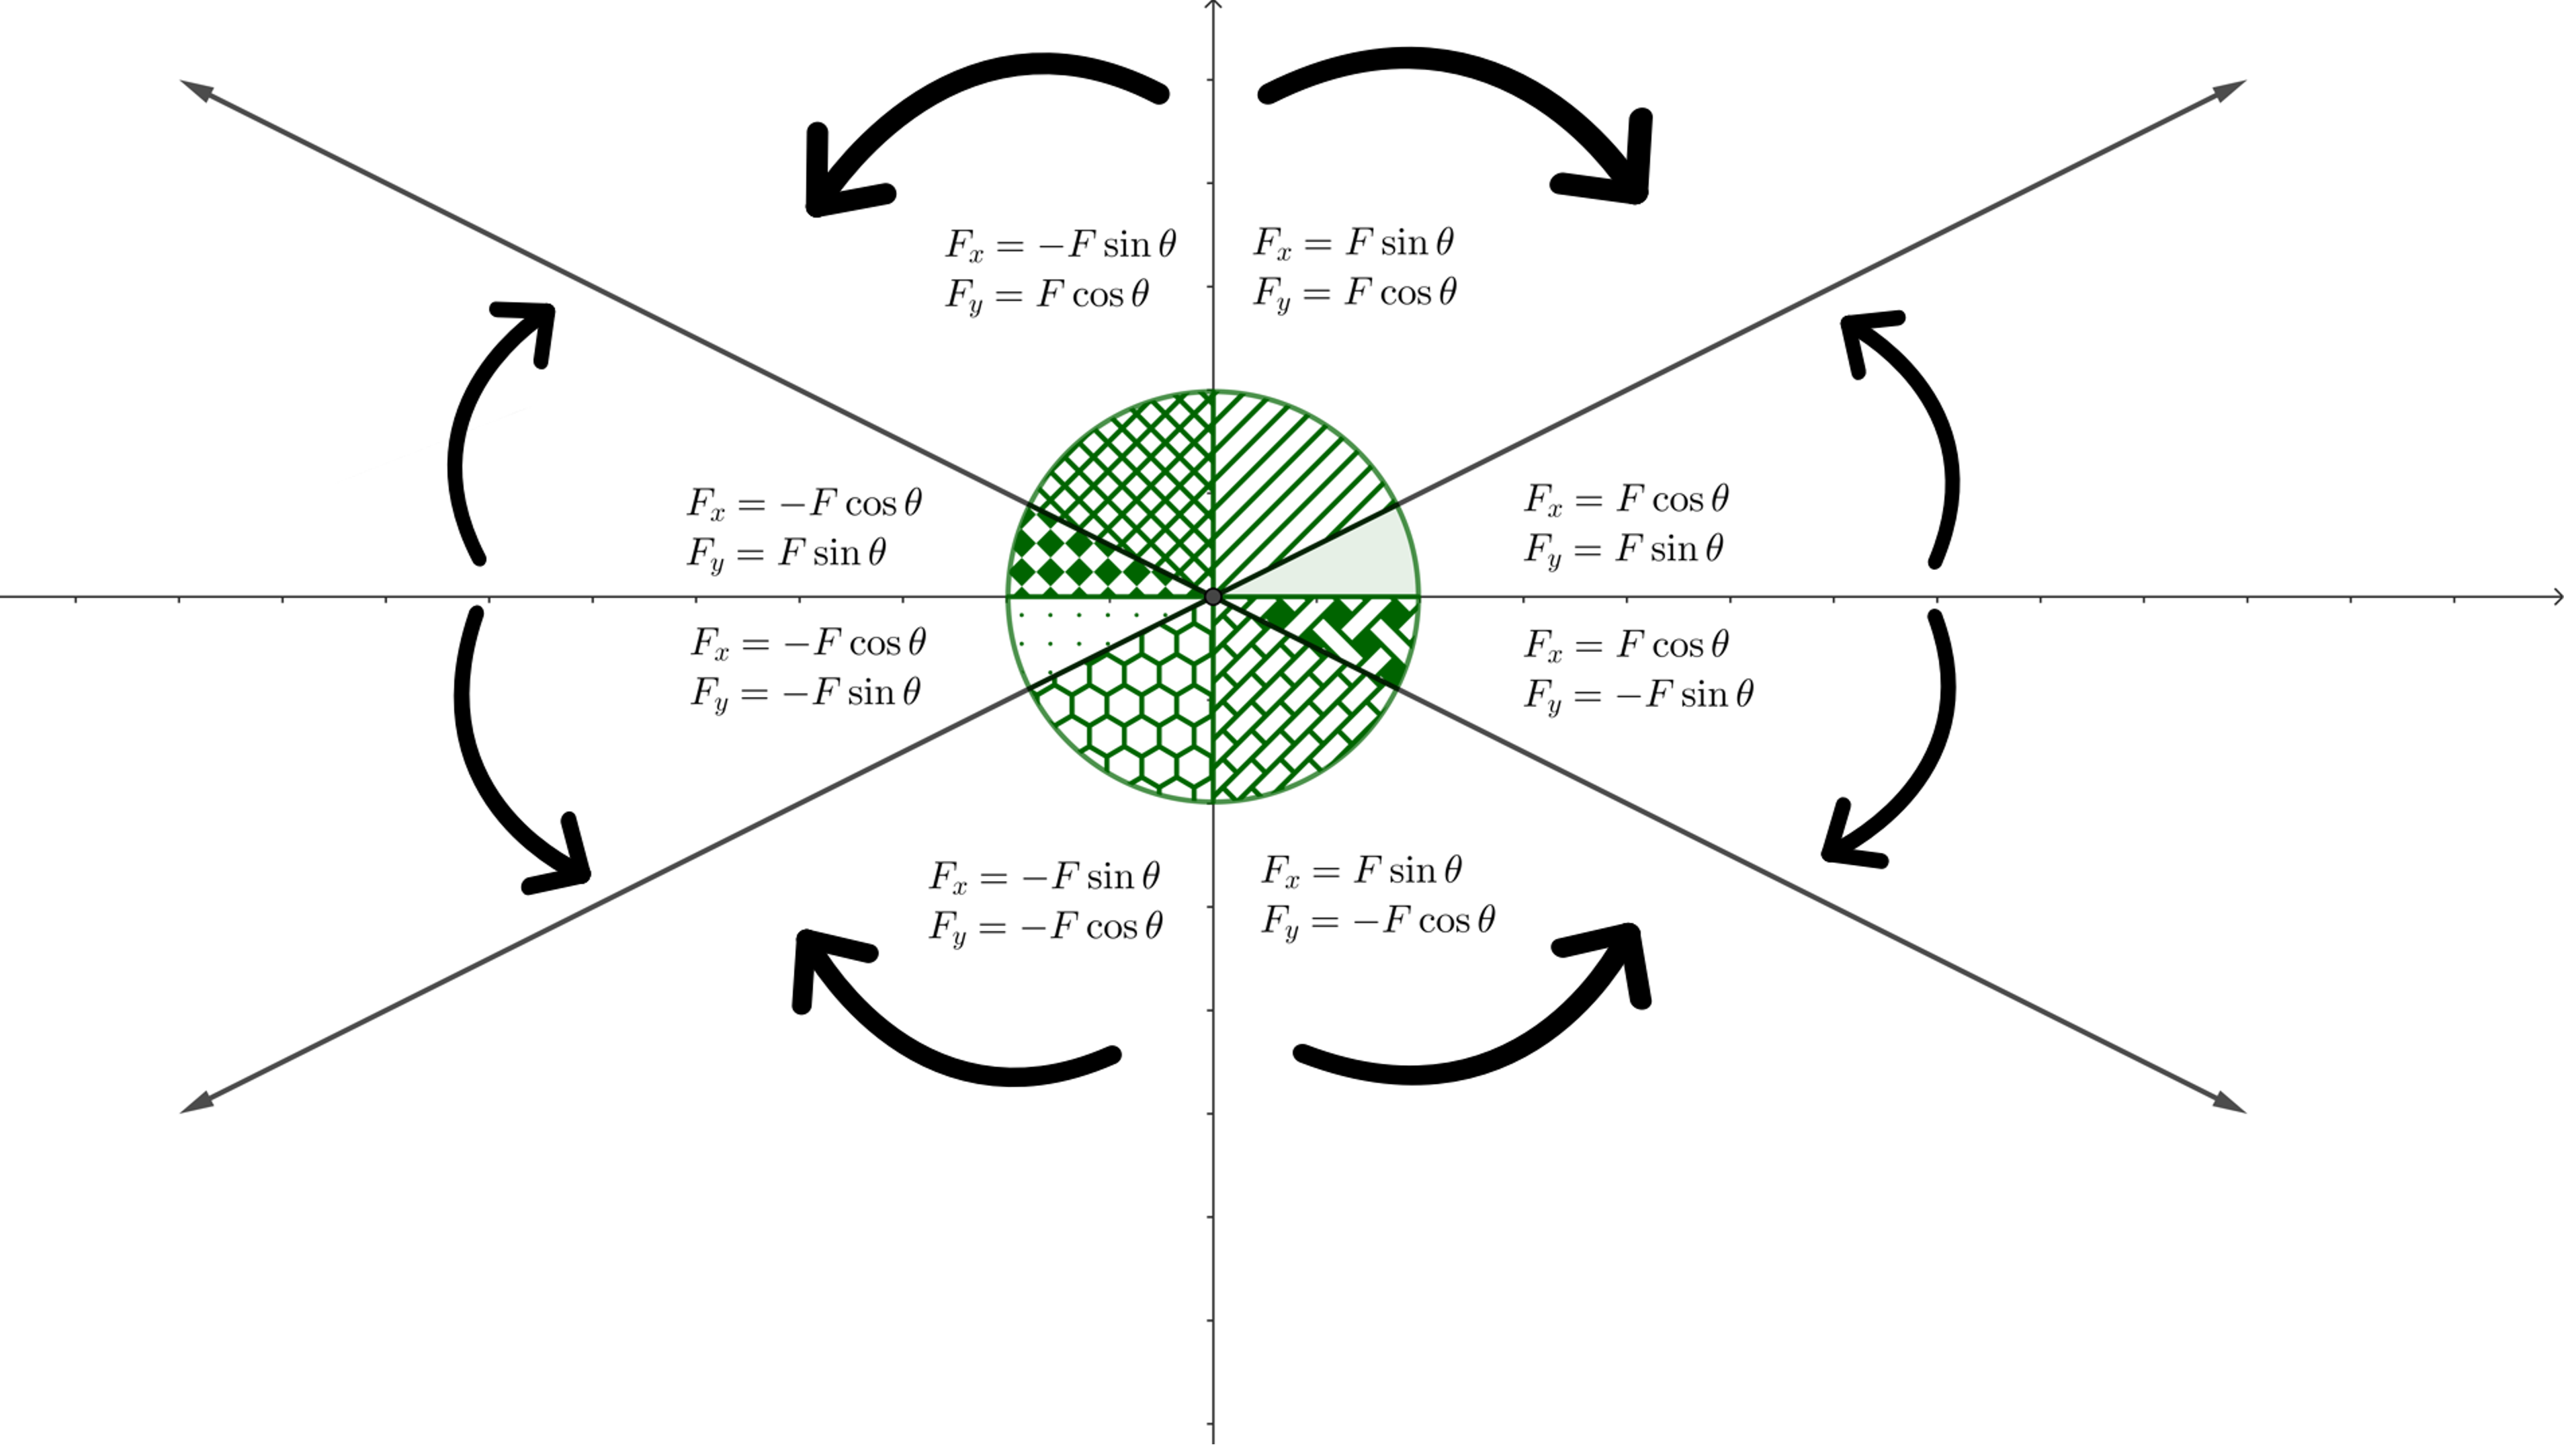
\includegraphics[width=0.8\textwidth]{Assets/Composants/Composants_w_arrows2.png}
    \caption{Komposanter kan findes efter vinkler fra forskellige akser}
    \label{komposanter}
\end{figure}

Givet vektoren $\vec A = A_x \hat i + A_y \hat j$, kan vektorens vinkel $\theta$ og størrelse $A$ findes ved:

\[
    A = \sqrt{A_x^2 + A_y^2} \hspace{6em}
    \theta = \arctan\left(\frac{A_y}{A_x}\right)
\]

Givet vektoren $\vec B$ med størrelse $B$ og vinkel $\phi$ fra den positive $x$-akse, kan vektorens komposanter $B_x$ og $B_y$ findes ved:
\[
    B_x = B \cos(\phi) \hspace{6em}
    B_y = B \sin(\phi)
\]

Generelt: Hvis komposanten man vil finde er \emph{hosliggende} ved vinklen, så bruges cosinus, hvis \emph{modstående}, så bruges sinus.
Se figur \ref{komposanter} for eksempel.

\subsection{Projektil-bevægelse}
2D bevægelse med konstant acceleration i $y$-retningen og 0 acceleration i $x$-retningen.

\subsubsection{Time of Flight}
Gælder kun hvis $y_0 = 0 = y_{\text{final}}$ \hfill $\theta_0$ er vinklen mellem $v_0$ og $x$.

\[
    T_{\text{tof}} = \frac{2 v_0 \sin(\theta_0)}{g}
\]

\bemærk{
    $T_{\text{tof}} \propto v_0$ og $T_{\text{tof}} \propto \frac{1}{g}$
}

\subsubsection{Trajectory}
\[
    y = \tan(\theta_0) \cdot x - \frac{g}{2(v_0 \cos(\theta_0))^2} \cdot x^2
\]

\bemærk{
    Ligningen er på formen $y= ax - bx^2$.
}

\subsubsection{Rækkevidde}
Givet at $x_0 = y_0 = 0$ og $y_{\text{final}} = 0$.
\[
    x = R = \frac{v_0^2 \sin(2\theta)}{g}
\]

\bemærk{
    $R \propto v_0^2$ og $R \propto \frac{1}{g}$.
}

Hvis $\theta_1 + \theta_2 = 90^\circ$ så er $R(\theta_1) = R(\theta_2)$.

\subsubsection{Top-punkt}

\[
    y_{\text{top}} = \frac{(v_0 \sin(\theta_0))^2}{2g}
\]


\subsection{Uniform Cirkulær bevægelse}
Bevægelse i en cirkel med konstant hastighed.

\subsubsection{Centripetal acceleration}

\[
    a_c = \frac{v^2}{r}
\]

Centripetal acceleration peger ind mod centrum af cirklen.

\subsubsection{Centripetal hastighed}
\[
    v = \frac{\text{Circumfrence}}{\text{Period}} = \frac{2\pi r}{T}
\]

\subsubsection{Positions-, hastigheds- og accelerationsvektorer}

\begin{minipage}
    {0.3\textwidth}
    \begin{align*}
        \text{Period of motion: } T &= \frac{2\pi r}{v} \\
        \text{Radius} = r & \\
        \text{Vinkelhastighed: } \omega &= \frac{2\pi}{T} = \frac{v}{r}
    \end{align*}
\end{minipage}
\hfill
\begin{minipage}
    {0.5\textwidth}
    \begin{align*}
        \vec r(t) &= r \cos(\omega t) \hat i + r \sin(\omega t) \hat j \\
        \vec v(t) &= -r\omega \sin(\omega t) \hat i + r\omega \cos(\omega t) \hat j \\
        \vec a(t) &= -r\omega^2 \cos(\omega t) \hat i - r\omega^2 \sin(\omega t) \hat j
    \end{align*}
\end{minipage}

\subsection{Non-uniform Cirkulær bevægelse}
Bevægelse i en cirkel med varierende hastighed, og dermed acceleration ud over den centripetale acceleration.

\subsubsection{Tangentiel acceleration}
\[
    a_T = \frac{d |\vec v|}{dt}
\]
Da $\vec a_T \perp \vec a_c$ gælder 
\begin{align*}
    \vec a_\text{total} &= \vec a_T + \vec a_c \\
    |\vec a_\text{total}| &= \sqrt{a_T^2 + a_c^2}
\end{align*}

\subsection{Relativ bevægelse}
Givet flere vektorer for det samme objekt i forskellige \textit{reference frames}, kan de samles:
\[
    \vec v_{AZ} = \vec v_{AB} + \vec v_{BC} + \vec v_{CD} + \ldots + \vec v_{YZ}
\]
Gælder både for position, hastighed og acceleration.